\section{Vector image model}\label{sec:SimpleRepModel}
The architecture for this model only contains fully connected layer, since the data representation only contains 21 element vector that reflects the active pain regions and gender as described in \autoref{LinetteAndBirgithe}. It's evaluated that there wouldn't be any gains in making the model more complex e.g. adding of convolution, based on the information available from vector, since the level of detail in relation to morphology is very simple. 
The architecture of the model is illustrated in \autoref{fig:simpleModel}. 

\begin{figure} [H]
\centering
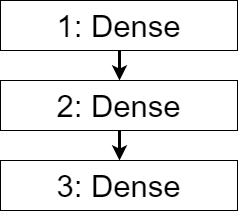
\includegraphics[width=0.3\textwidth]{figures/simpleModel}
\caption{Arcitechture of the neural network using knee region representation.}
\label{fig:simpleModel}  
\end{figure}

The model consists of three layers, where the input and output layer... 



\section{Raw binary representation model}\label{sec:BinaryRepModel}
The architecture of this model is based on the typical structure of a convolutional network, where the first layers alternate between convolutional layers and max pooling layers \citep{LeCun2015}. This defines the first part of the model. The following layers consists of three fully connected layers, and output layer, and defined the second part of the model. An overview of the architecture is shown in \autoref{fig:binaryRepModel}.  
Convolution layer are implemented for this pain map representation, because of their ability to extract morphology features from images, as written in \autoref{CONVOLUTION}

\begin{figure} [H]
\centering
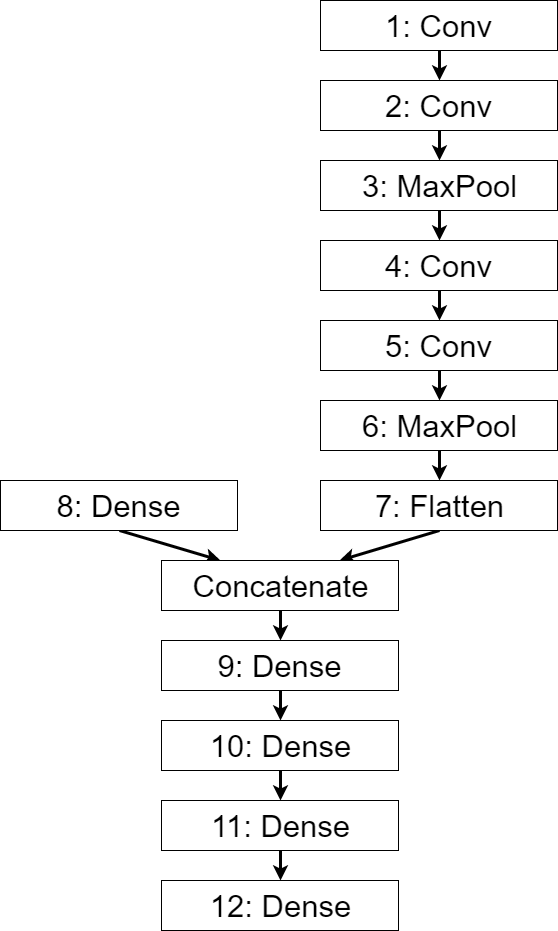
\includegraphics[width=0.6\textwidth]{figures/binaryRepModel}
\caption{Architecture for the neural network model using binary pain map representation. REMEMBER TO INCLUDE THE INPUT IN THE FIGURE}
\label{fig:binaryRepModel}  
\end{figure}

Rather then feeding both pain map representation and gender into the same input layer, they are separated and used as input at two different locations. 
The binary pain map representation works as input in first part of the model, where the input layer is a convolution layer. 
This layer is setup to receive a input shape to that of the dimension of the pain map, that is defined during re-scaleing of the pain maps in \ref{LINETTE&BIRGITHE}. 
Gender works as secondary input in the second section of the model, along with the pain maps features extracted through the convolution layers. Before the pain maps features reach the fully connected part of the network it is flattened from a matrix to a single row in order to merge the features with gender. 
The merged data passes the fully connected layers and reaches the output layer where it is given a percentage value according to which class it fits the most.
The second part of the model resembles the simple representation model, described in \ref{sec:SimpleRepModel} 


THIS NEEDS TO BE REWRITTEN: The reason for separating gender and binary images is given as separate inputs is because of that there is no benefit in feeding gender through several convolutional layers, since these layer are use for looking at the shapes of the pain.  

The reason for using gender as input this far into the model, is a result of the way that convolution works 


\section{Combined representation model}\label{sec:CombinedRepModel}
The architecture of this model is nearly identical to that of the binary representation model as described in \ref{sec:BinaryRepModel}. 
The main difference can only be seen in the input layer for the pain map representation, where the input shape is altered to contain 20 layers per pain maps instead of one. 
This is the result of the one hot encoding done to the images as described in \autoref{LinetteAndBirgithe}. 

%\begin{figure} [H]
%\centering
%\includegraphics[width=0.6\textwidth]{figures/XXX}
%\caption{}
%\label{fig:CombinedRepModel}  
%\end{figure}
